\documentclass[a4paper, fontsize=14pt]{article}
\usepackage{scrextend}
\usepackage{indentfirst, fancyhdr, amsfonts, mathtools, amssymb}
\usepackage{titlesec} %работа с рубрикацией
\usepackage{tocloft} %настройки оглавления
\usepackage[T2A]{fontenc}
\usepackage[utf8x]{inputenc}
\usepackage[russian]{babel}
\usepackage{hyperref} %кликабельное оглавление
\usepackage[left=3.7cm,right=2cm,top=2cm,bottom=2cm]{geometry}
\usepackage{tempora} %настраиваем шрифт типа TNR                                   
\usepackage{newtxmath} %делаем шрифт формул похожим на TNR
\usepackage{caption}
\usepackage{pdfpages}
\usepackage{listings}
\lstset{
  columns=fullflexible,
  breaklines=true,
}
\linespread{1}
\setcounter{page}{4} %в зависимости от того, какой по счёту страницей должно быть оглавление!

%НАСТРОЙКИ ОГЛАВЛЕНИЯ
\renewcommand{\cftsecaftersnum}{.} %точки после номеров разделов и подразделов в оглавлении
\renewcommand{\cftsubsecaftersnum}{.}
\renewcommand{\cftsecfont}{\normalfont} %разделы в оглавлении пишутся обычным (не жирным) шрифтом
\renewcommand{\cftsecpagefont}{\normalfont} %соответствующие им страницы тоже
\renewcommand{\cftsecleader}{\cftdotfill{\cftdotsep}} %расставляем точки между названиями разделов и их страницами
\addto\captionsrussian{\renewcommand\contentsname{СОДЕРЖАНИЕ}} %хотим, чтобы слово "Содержание" писалось капсом
\renewcommand{\cfttoctitlefont}{\hfil\bfseries} %слово СОДЕРЖАНИЕ по центру жирным
\renewcommand{\cftaftertoctitle}{\hfill}

%НАСТРОЙКИ РУБРИКАЦИИ
\titleformat*{\section}{\center\bf} %названия разделов и подразделов по середине жирным шрифтом
\titleformat*{\subsection}{\center\bf}
\titlelabel{\thetitle.\quad} %название раздела и его номер отделены точкой

%НАСТРОЙКИ БИБЛИОГРАФИИ
\addto\captionsrussian{\renewcommand\refname{СПИСОК ЛИТЕРАТУРЫ}} %хотим, чтобы слова "Список литературы" писались капсом
\makeatletter
\renewcommand{\@biblabel}[1]{#1.} %хотим, чтобы в списке литературы номера источников писались в формате "No. <...>", а не "[No] <...>"
\makeatother

\begin{document}
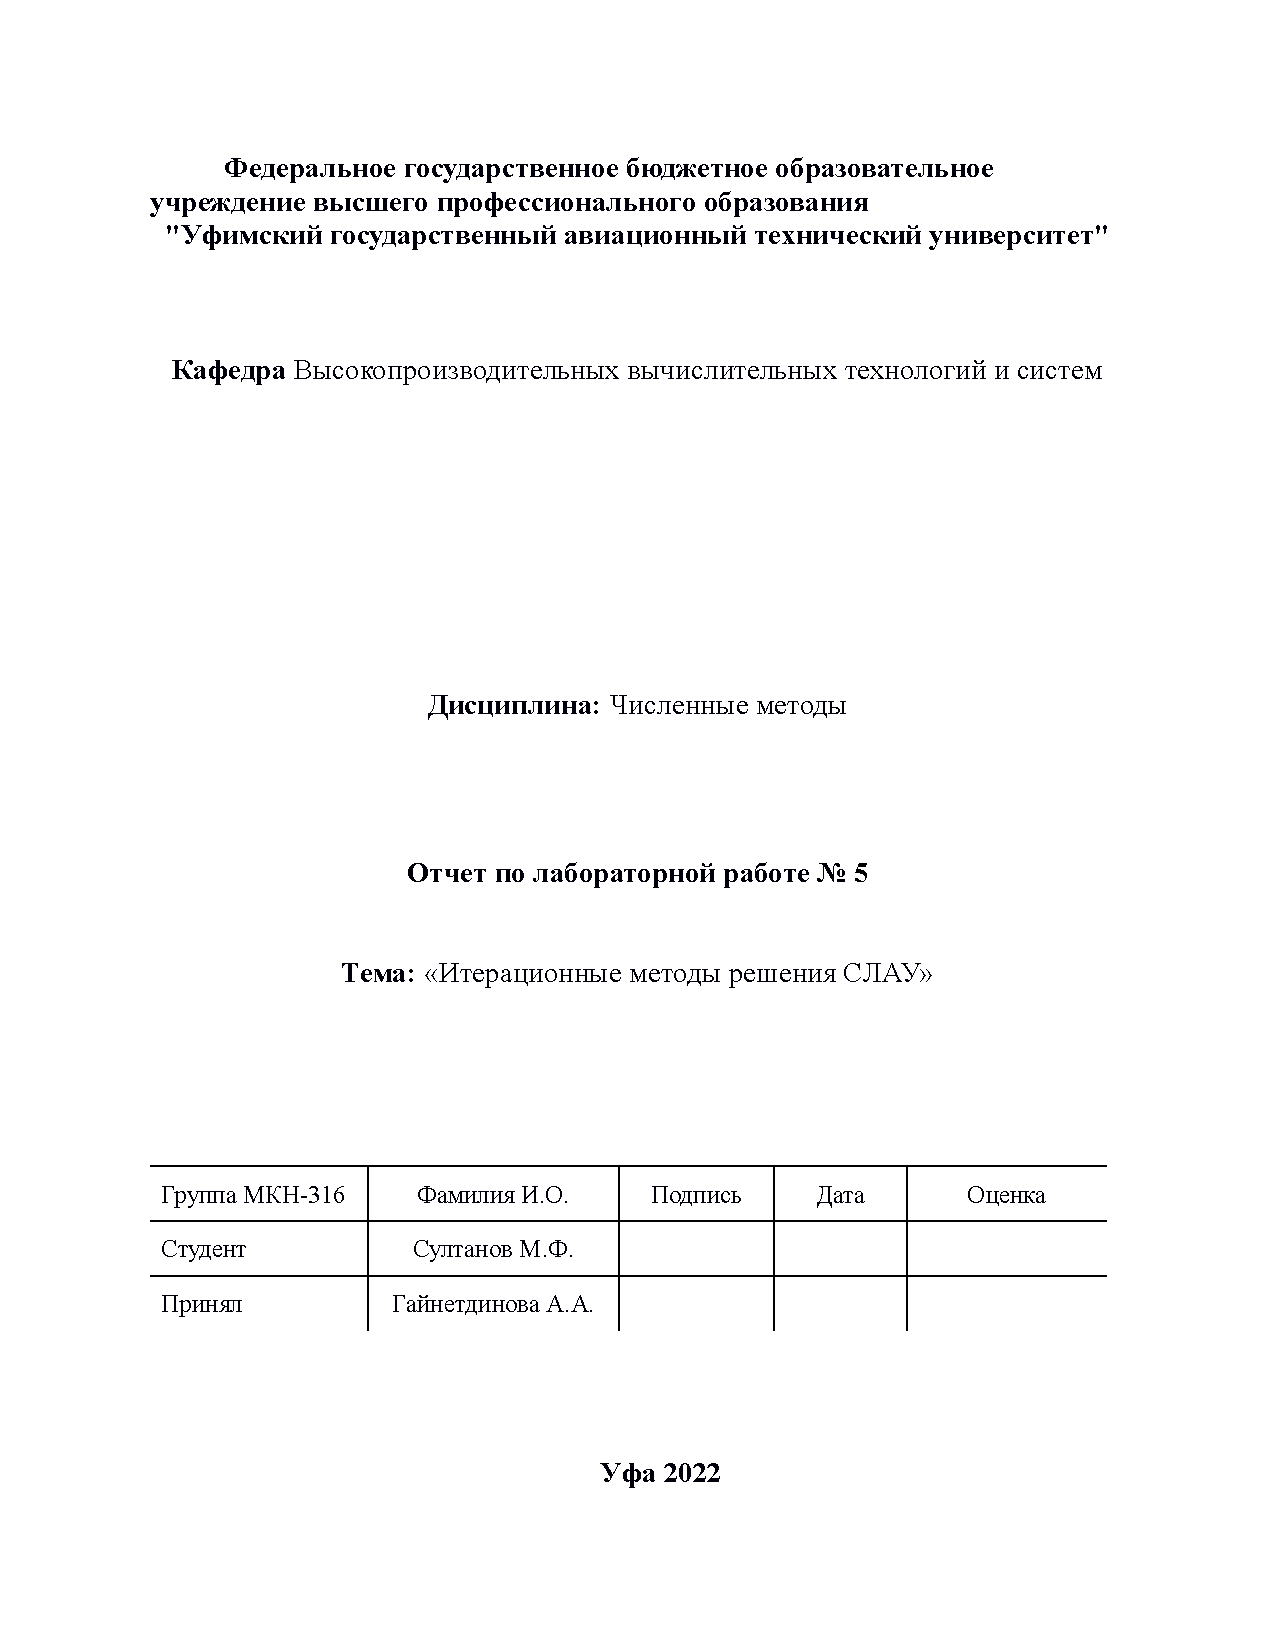
\includepdf[pages={1}]{src/front_page.pdf}
\textbf{Цель работы:}  получить навык проведения вычислительного
эксперимента, направленного на исследование свойств итерационных методов
решения СЛАУ.
\subsection*{{Ход работы}}
\subsubsection*{Задача №1}
Сгенерировать симметричную ленточную матрицу размера $N \times N$ с шириной ленты $4l + 1$ и обладающую диагональным преобладанием.
\subsubsection*{Решение}

Алгоритм,приведенный в условии задачи, в общем случае, не генерирует матрицу с диагональным преобладанием. Пример при расчетах в Maple продемонстрирован на рисунке \ref{fig:incorrent_ex1}.
\begin{center}
    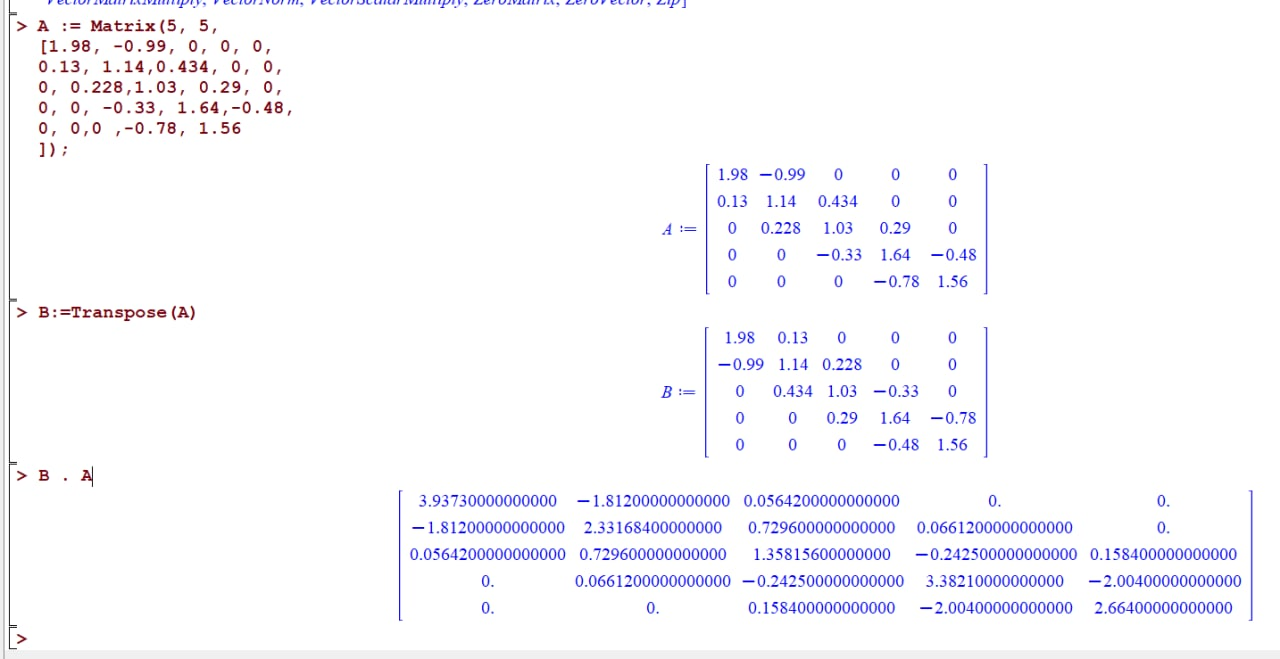
\includegraphics[scale=0.5]{src/incorrent_ex1.png}
    \captionof{figure}{Пример матрицы без диагонального преобладания}
    \label{fig:incorrent_ex1}
\end{center}

Был реализован алгоритм, который сразу построчно генерирует ленточную матрицу указанного вида. Кроме того, была реализована система хранения матриц $A$, 
которая позволяет по индексации исходной матрицы взаимнооднозначно получить элемент матрицы $A$ и не хранит нулевые элементы.
\begin{equation*}
    a_{ij} = A(2l + 1 + i - j , j), \quad max(1, j - 2l) \leq i \leq j
\end{equation*}

Например, для матриц $N = 5, l = 1$:
\begin{equation*}
    \{a_{ij}\} = \begin{pmatrix}
        a_{11} & a_{12} & a_{13} & 0      & 0 \\
        a_{12} & a_{22} & a_{23} & a_{24} & 0 \\
        a_{13} & a_{23} & a_{33} & a_{34} & a_{35} \\
        0      & a_{24} & a_{34} & a_{44} & a_{45} \\
        0      & 0      & a_{35} & a_{45} & a_{55}
    \end{pmatrix}
\end{equation*}
\begin{equation*}
    A(i, j) = \begin{pmatrix}
        * & * & a_{13} & a_{23} & a_{35} \\
        * & a_{12} & a_{23} & a_{34} & a_{45} \\
        a_{11} & a_{22} & a_{33} & a_{44} & a_{55}
    \end{pmatrix}
\end{equation*}


\subsubsection*{Задача №2. Метод Якоби}
\begin{enumerate}
    
    \item Написать вычислительную программу на языке программирования C++
    для решения СЛАУ с указанной в индивидуальном задании точностью
    методом Якоби, являющегося частным случаем метода простых
    итераций.
    \item С использованием написанной программы исследовать зависимость
    числа итераций метода Якоби, необходимых для достижения заданной
    точности, от величины параметра $q$, определяющего степень
    диагонального преобладания.
\end{enumerate}
\subsubsection*{Решение}

\begin{center}
    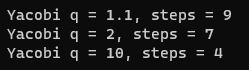
\includegraphics[]{src/yacobi.png}
    \captionof{figure}{Результат работы программы, реализующей метод Якоби}
    \label{fig:yacobi}
\end{center}

Таким образом, при большей обусловленности матрицы метод Якоби сходится быстрее.

\subsubsection*{Задача №3. Метод SOR}
\begin{enumerate}
    
    \item Написать вычислительную программу на языке программирования C++
    для решения СЛАУ с указанной в индивидуальном задании точностью
    методом последовательной верхней релаксации (SOR) с параметром
    релаксации $\omega\in(0,2)$.
    \item С использованием написанной программы исследовать зависимость
    числа итераций метода SOR от параметров $q$ и $\omega$. При сравнении
    предусмотреть частный случай $\omega = 1$, соответствующий методу Гаусса-Зейделя.
диагонального преобладания.
\end{enumerate}
\subsubsection*{Решение}
\begin{center}
    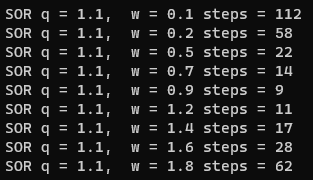
\includegraphics[]{src/sor11.png}
    \captionof{figure}{Результат работы программы, реализующей метод SOR при $q = 1.1$}
    \label{fig:sor11}
\end{center}


\begin{center}
    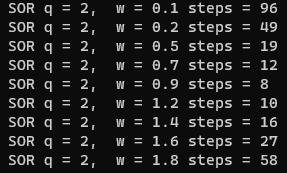
\includegraphics[]{src/sor2.png}
    \captionof{figure}{Результат работы программы, реализующей метод SOR при $q = 2$}
    \label{fig:sor2}
\end{center}

\begin{center}
    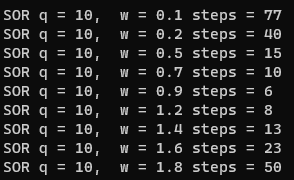
\includegraphics[]{src/sor10.png}
    \captionof{figure}{Результат работы программы, реализующй метод SOR при  $q = 10$}
    \label{fig:sor10}
\end{center}

\begin{center}
    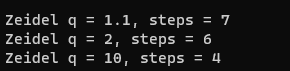
\includegraphics[]{src/zeidel.png}
    \captionof{figure}{Результат работы программы, реализующй метод Зейделя}
    \label{fig:zeidel}
\end{center}

Таким образом, наиболее оптимальным алгоритмом является метод Зейделя $\omega = 1$ при наибольшем диагональном преобладании.


\subsubsection*{Задача №3. Метод PCGM}
\begin{enumerate}
    \item Написать вычислительную программу на языке программирования C++
    для решения СЛАУ с указанной в индивидуальном задании точностью
    методом сопряженных градиентов (CGM).
    \item  С использованием написанной программы исследовать зависимость
    числа итераций метода сопряженных градиентов от параметра $q$.
    \item  Выполнить модификацию написанной программы путем введения
    предобуславливателя в виде m-шагового метода Якоби.
    \item  Для системы с матрицей $A_i$, требующей наибольшего числа итераций
    метода сопряженных градиентов, с использованием написанной
    программы исследовать зависимость числа итераций метода
    сопряженных градиентов с предобуславливателем (PCGM) от количества
    шагов $m$ метода Якоби, используемого в качестве предобуславливателя.
\end{enumerate}
\subsubsection*{Решение}

\begin{center}
    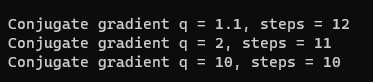
\includegraphics[]{src/conjugate}
    \captionof{figure}{Результат работы программы, реализующй CGM}
    \label{fig:conjugate}
\end{center}
\begin{center}
    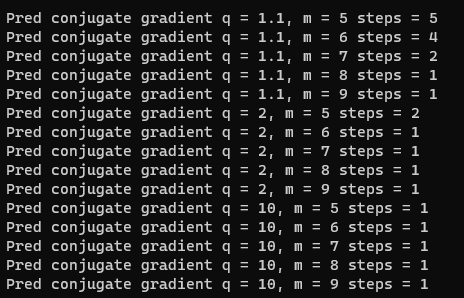
\includegraphics[]{src/predconj.png}
    \captionof{figure}{Результат работы программы, реализующй PCGM с предобуславливателем метода Якоби}
    \label{fig:conjugate}
\end{center}    \newpage
\section*{{Вывод}}
Вьходе лабораторной работы был получен навык проведения вычислительного
эксперимента, направленного на исследование свойств итерационных методов
решения СЛАУ.
\newpage
\subsection*{Список литературы}
\begin{enumerate}
    \item Бахвалов Н.С., Жидков Н.П., Кобельков Г.М. Численные методы: Бином, 2018. – 636 с. 
    \item Калиткин Н.Н. Численные методы, 2-е издание: БХВ-Петербург, 2014. – 592 с.
    \item Самарский А.А., Гулин А. В. Численные методы: Учеб, пособие для вузов, — М.: Наука. Гл. ред. физ-мат. лит., 1989.— 432 с.
\end{enumerate}
\newpage
\subsection*{Приложение}
Весь С++ код выложен в github-репозитории по ссылке: 

\url{https://github.com/sultanovMF/Numerical-Methods-Lab}


\end{document}